\chapter{Antecedentes de probabilidad}

\section{Definiciones iniciales}

Un \emph{experimento causal, indeterminista o de azar} es aquel para el cual no necesariamente podemos predecir con certeza lo que va a ocurrir al realizarlo.  Cuando se repite el mismo experimento bajo las mismas condiciones se puede obtener un resultado diferente.
\begin{quotation}
 Ej: ``predecir el resultado de lanzar dos monedas.''
\end{quotation}

\begin{description}
 \item [Evento simple.] Cualquier resultado elemental de un experimento aleatorio.
  \begin{quotation}
   Ej: a: ``obtener el 2 al lanzar un dado.''
  \end{quotation}
  
 \item [Evento.] Cualquier conjunto de resultados posibles de un experimento aleatorio.
  \begin{quotation}
   Ej: A: ``obtener un par al lanzar un dado.''
   
       $A = \{2,4,6\} = \{$ ``obtengo el dos'', ``o... cuatro'', ``o... seis''$\} = \{x|x=2,4,6\}$
  \end{quotation}
  
 \item [Espacio de eventos, muestras o Universo $S$.]  Conjunto de todos los eventos simples posibles en un experimento aleatorio.
  \begin{quotation}
   Ej: ``lanzar un dado.''
   
       $S = \{1,2,3,4,5,6\}$
  \end{quotation}
 \item [Tamaño de un evento.] Número de eventos simples que satifacen la definición del evento (cardinalidad del conjunto).
 \begin{quotation}
  Ej: tamaño de A: $|A| = 3$.
 \end{quotation}
\end{description}

\begin{definition}
Definimos a la probabilidad de un evento $A$ como:
\begin{align}
 P(A) =& \dfrac{|A|}{|S|}. \label{eq:proba_laplace}
\end{align}

Destaca también lo que se conoce como la \emph{definición frecuentista} de probabilidad, en la cual esta cantidad $P(A)$ se define con respecto a una secuencia potencialmente infinita de repeticiones del experimento aleatorio $A$.
\end{definition}

Es posible representar gráficamente a los eventos utilizando \emph{diagramas de Venn}.  Por ejemplo, sea $S$ el Universo y $A$ un evento, su diagrama correspondiente se muestra en la \fref{fig:venn_a}.

\begin{figure}
  \centering
  \def\firstcircle{(0,0) circle (1.5cm)}
  \def\universesquare{(-3,-2) rectangle (3,2)}
  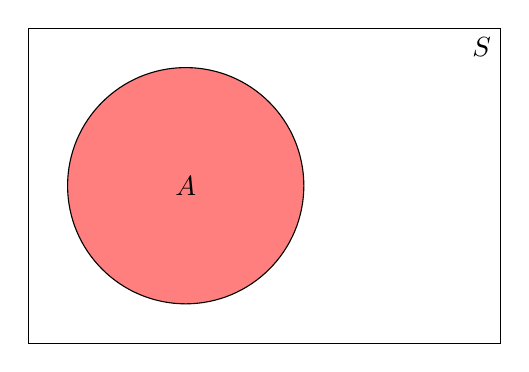
\begin{tikzpicture}
      \begin{scope}[fill opacity=0.5]
	  \fill[red] \firstcircle;
	  \draw \firstcircle [opacity=1] node {$A$};
	  \draw \universesquare [opacity=1] node [below left] {$S$};
      \end{scope}
  \end{tikzpicture}
  \caption{Evento $A$ en el espacio de eventos $S$.}\label{fig:venn_a}
\end{figure}

Se dice que dos eventos son \emph{mutuamente exclusivos} si no pueden ser verdad al mismo tiempo y se pueden visualizar como dos conjuntos ajenos \fref{fig:exclusivos}.

\begin{figure}
  \centering
  \def\firstcircle{(-1.25,0) circle (1cm)}
  \def\secondcircle{(1.25,0) circle (1cm)}
  \def\universesquare{(-3,-2) rectangle (3,2)}
  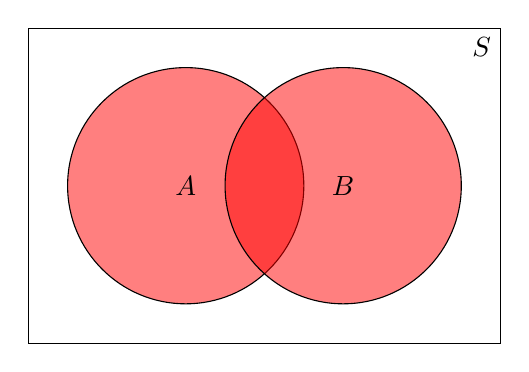
\begin{tikzpicture}
      \begin{scope}[fill opacity=0.5]
	  \fill[red] \firstcircle;
	  \draw \firstcircle [opacity=1] node {$A$};
	  \fill[red] \secondcircle;
	  \draw \secondcircle [opacity=1] node {$B$};
	  \draw \universesquare [opacity=1] node [below left] {$S$};
      \end{scope}
  \end{tikzpicture}
  \caption{Eventos mutuamente exclusivos $A$ y $B$ en el espacio de eventos $S$.}\label{fig:exclusivos}
\end{figure}

Eventos posibles incluyen al universo $S$ y al conjunto que no contiene resultados $\phi$.  Dados dos eventos $E$ y $F$ es posible crear otros eventos mediante las operaciones:

\begin{figure}
  \centering
  \def\firstcircle{(0,0) circle (1.5cm)}
  \def\secondcircle{(0:2cm) circle (1.5cm)}
  \def\universesquare{(-2,-2) rectangle (4,2)}
  \def\universesmall{(-2,-2) rectangle (2,2)}
  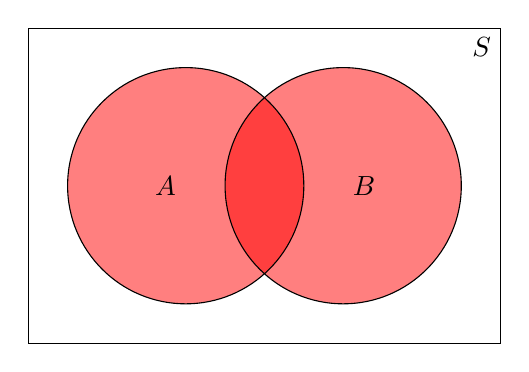
\begin{tikzpicture}
      \begin{scope}[fill opacity=0.5]
	  \fill[red] \firstcircle;
	  \fill[red] \secondcircle;
	  \draw \firstcircle [opacity=1] node [left] {$A$};
	  \draw \secondcircle [opacity=1] node [right] {$B$};
	  \draw \universesquare [opacity=1] node [below left] {$S$};
      \end{scope}
  \end{tikzpicture}
  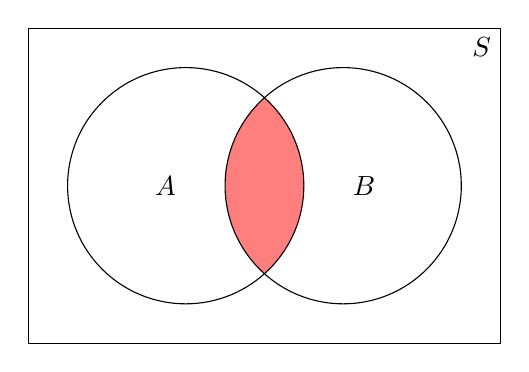
\begin{tikzpicture}
      \begin{scope}[fill opacity=0.5]
	\begin{scope}
	  \clip \firstcircle;
	  \fill[red] \secondcircle;
	\end{scope}
	  \draw \firstcircle [opacity=1] node [left] {$A$};
	  \draw \secondcircle [opacity=1] node [right] {$B$};
	  \draw \universesquare [opacity=1] node [below left] {$S$};
      \end{scope}
  \end{tikzpicture}
  
  \vspace{2mm}
  \begin{tikzpicture}
      \begin{scope}[fill opacity=0.5]
	  \fill[red] \universesmall;
	  \fill[white, opacity=1] \firstcircle;
	  \draw \firstcircle [opacity=1] node {$A$};
	  \draw \universesmall [opacity=1] node [below left] {$S$};
      \end{scope}
  \end{tikzpicture}
  \caption{Arriba izquierda: Unión de eventos.  Arriba derecha: Intersección.  Abajo: Complemento.}\label{fig:creacionEventos}
\end{figure}

\begin{description}
 \item [Unión.] La unión de dos eventos $E \cup F$ es el conjunto de eventos simples en $E$ o $F$ inclusivamente. \fref{fig:creacionEventos} (Izquierda).
 \item [Intersección.]  La intersección de dos eventos $E \cap F$ es el conjunto de eventos simples en ambos $E$ y $F$ al mismo tiempo. \fref{fig:creacionEventos} (Derecha).
 \item [Complemento.] El complemento de un evento es el conjunto de los eventos simples que no se encuentran en $E$, denotado $\bar{E}$.
\end{description}



\section{Variable aleatoria}

Una variable aleatoria es una función que va del espacio de muestras a los reales $X : S \rightarrow \mathbb{R}$\footnote{Por convensión, escribiremos las variables aleatorias con mayúsculas y sus valores concretos con minúsculas.}.  Esta función permite medir el aspecto de interés para un evento dado, en función de los resultados elementales obtenidos. 
  \begin{quotation}
   Ej: Para el evento E:``obtener un 7 al lanzar dos dados''.
   
       Sea la variable aleatoria $X$ : ``La suma del resultado en cada uno de dos dados''.
   
       $X(dado_1, dado_2) = dado_1 + dado_2$
       
       Entonces el evento $E$ se expresa como $E : X(dado_1, dado_2) = 7$.
  \end{quotation}
Obsérvese que la función de la variable aleatoria puede ser, como un caso particular, la función identidad si el espacio de eventos está contenido en los reales.  Otro caso particular sería una función que realice un mapeo uno a uno del espacio de eventos hacia los reales.  Para ello es necesario que los valores en el dominio sean:
 \begin{enumerate}
  \item Mutuamente exclusivos.
  \item Exhaustivos.
 \end{enumerate}

 \begin{quotation}
  Ej: Formalmente la variable aleatoria $C(Clima)$ tendría el rango:
  \begin{align*}
   C(Clima) = <1, 2, 3, 4, 5>
  \end{align*}
 
  Dichos valores podrían venir de un mapeo directo con los valores del espacio de eventos:
   \begin{align*}
    Clima =& <despejado, lluvioso, nublado, granizado, nevado> \\
    C(Clima) =& \begin{cases}
		1	& \text{si } despejado \\
		2       & \text{si } lluvioso \\
		3	& \text{si } nublado \\
		4	& \text{si } granizado \\
		5	& \text{si } nevado
	      \end{cases}
   \end{align*}
   
   Esto también se puede escribir $C \in \{c^1,c^2,c^3,c^4,c^5\}$, que abrevia los casos $C=1,C=2,C=3,C=4,C=5$.
 \end{quotation}

 
De este modo es posible asociar una variable aleatoria a cada variable natural del espacio de eventos.  Por comodidad y legibilidad, frecuentemente se hará referencia a la variable del espacio de eventos como una \textit{variable aleatoria}, con un dominio diferente a los reales, aunque formalmente debe sobre-entenderse la existencia de un mapeo entre los elementos del espacio de eventos y los número reales.

\subsection{Variables aleatorias discretas y continuas}

Es posible clasificar a las variables aleatorias de acuerdo a las características de su rango en:
\begin{description}
 \item [Discretas.] Su rango consiste en un número finito de valores.
 
 Un caso particular de variables discretas son las variables booleanas, donde los valores que pueden tomar son $\{0,1\}$.
 
 Es posible asignar una probabilidad a cada valor de una variable aleatoria discreta, definiendo lo que será entonces una \emph{distribución de probabilidad}.  Dado que los valores de la variable aleatoria son exclusivos, la suma de las probabilidades sobre todos los valores debe ser $1$.

 \begin{quotation}
  Ej:
  \begin{align*}
   P(Clima) =&  \begin{cases}
		0.4	& \text{si } despejado \\
		0.25       & \text{si } lluvioso \\
		0.15	& \text{si } nublado \\
		0.1	& \text{si } granizado \\
		0.1	& \text{si } nevado
	      \end{cases}
  \end{align*}

 \end{quotation}
 
 \item [Continuas.] Al realizar un experimento aleatorio todos los valores sobre $\mathbb{R}$ o un intervalo $[a,b] \in \mathbb{R}$ son resultados posibles.
 \begin{quotation}
  Ej: ``$Temperatura \in [0,60000]\degree K$''.
 \end{quotation}
  Dado que el número de elementos en un intervalo continuo es infinito, la probabilidad de obtener un valor específico es cero.  Por consiguiente se define una \emph{función de densidad de probabilidad}\footnote{Obsérvese que, en principio, $f(x)$ puede tomar valores mayores que uno \cite{Barber2012}.}
  \begin{align}
   f(x) &\geq 0
  \end{align}
  a partir de la cual se calcula la probabilidad de que $X$ tome algún valor dentro de un subconjunto mesurable $B \in \mathbb{R}$ de sus valores posibles:
  \begin{align}
   P(X \in B) &= \int_B f(x) dx
  \end{align}
  En particular, si $B$ es un intervalo de $\mathbb{R}$ entonces:
  \begin{align}
   P(a \leq X \leq b) = \int_a^b f(x) dx
  \end{align}
  Dado que $X$ debe tomar algún valor en $\mathbb{R}$, entonces $P(X)$ debe satisfacer:
  \begin{align}
   P(X \in (-\infty,\infty)) = \int_{-\infty}^{\infty} f(x) dx = 1
  \end{align}
\end{description}

\subsection{Extensión de la lógica proposicional}
 
Es posible utilizar la teoría de probabilidades para extender a la lógica proposicional.  El tipo más sencillo de proposición a utilizar es la afirmación de que una variable aleatoria tiene un valor particular tomado de su dominio.
\begin{quotation}
 Ej: ``$Temperatura = 310$''.
\end{quotation}
Dicho esto, es posible asociar una probabilidad al evento de que una proposición dada sea verdadera o falsa.  Gracias a ello será posible realizar inferencias en condiciones de incertidumbre.


\section{Axiomas de la probabilidad}

Andrei Kolmogorov demostró cómo desarrollar el resto de la teoría probabilista a partir de los tres axiomas que llevan su nombre\footnote{\cite{Russell2004}}:

\begin{enumerate}
 \item Todas las probabilidades están entre 0 y 1. Para cualquier proposición $a$,
 \begin{equation}
  0 \leq P(a)\leq 1
 \end{equation}
 
 \item Las proposiciones necesariamente ciertas (es decir, válidas) tienen probabilidad 1, y las proposiciones necesariamente falsas (es decir, insatisfacibles) tienen probabilidad 0.
 \begin{align}
  P(cierto) =& 1 & P(falso) =& 0
 \end{align}
 
 \item La probabilidad de una disyunción viene dada por
 \begin{equation}
  P(a \lor b) = P(a) + P(b) - P(a \land b)
 \end{equation}
\end{enumerate}

\begin{figure}
  \centering
  \def\firstcircle{(0,0) circle (1.5cm)}
  \def\secondcircle{(0:2cm) circle (1.5cm)}
  \def\universesquare{(-2,-2) rectangle (4,2)}
  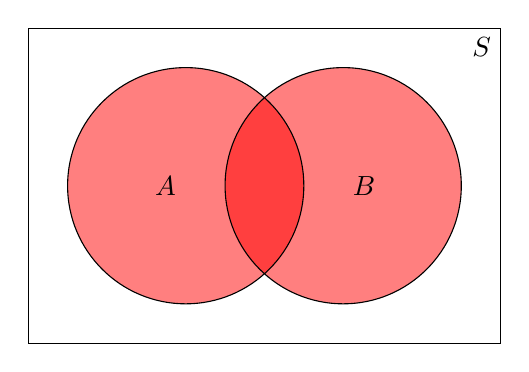
\begin{tikzpicture}
      \begin{scope}[fill opacity=0.5]
	  \fill[red] \firstcircle;
	  \fill[red] \secondcircle;
	  \draw \firstcircle [opacity=1] node [left] {$A$};
	  \draw \secondcircle [opacity=1] node [right] {$B$};
	  \draw \universesquare [opacity=1] node [below left] {$S$};
      \end{scope}
  \end{tikzpicture}
  \caption{La probabilidad $P(a \lor b)$ corresponde a la probabilidad de la unión de ambos eventos.}\label{fig:p_or}
\end{figure}

Este último axioma es fácilmente interpretable utilizando teoría de conjuntos \fref{fig:p_or}, pues utilizando la \eref{eq:proba_laplace} se tiene:

\begin{align*}
 P(a \lor b) = \dfrac{|a \cup b|}{|S|} = \dfrac{|a| + |b| - |a \cap b|}{|S|} = P(a) + P(b) - P(a \land b).
\end{align*}



\section{Probabilidad condicional}

\begin{figure}
  \centering
  \def\firstcircle{(0,0) circle (1.5cm)}
  \def\secondcircle{(0:2cm) circle (1.5cm)}
  \def\universesquare{(-2,-2) rectangle (4,2)}
  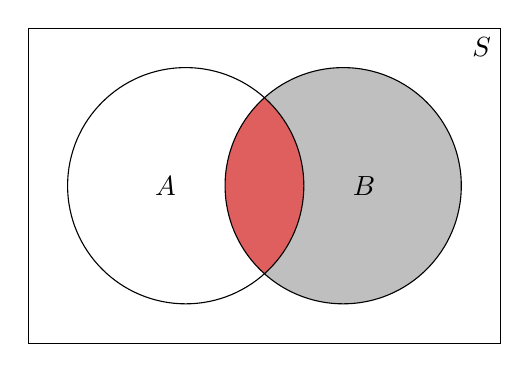
\begin{tikzpicture}
      \begin{scope}[fill opacity=0.5]
        \fill[gray] \secondcircle;
	\begin{scope}
	  \clip \firstcircle;
	  \fill[red] \secondcircle;
	\end{scope}
	  \draw \firstcircle [opacity=1] node [left] {$A$};
	  \draw \secondcircle [opacity=1] node [right] {$B$};
	  \draw \universesquare [opacity=1] node [below left] {$S$};
      \end{scope}
  \end{tikzpicture}
  \caption{La probabilidad $P(a | b)$ corresponde a la probabilidad de la intersección de ambos eventos, como si $B$ fuera el nuevo universo.}\label{fig:p_cond}
\end{figure}

Es posible definir la probabilidad de un evento sujeto a la evidencia observada como (\fref{fig:p_cond}):
\begin{align}
 P(a|b) = \dfrac{P(a \land b)}{P(b)} \label{eq:p_cond}
\end{align}

\section{Teorema de Bayes}

Si tomamos las definiciones de probabilidad condicional:
\begin{align}
 P(a|b) &= \dfrac{P(a \land b)}{P(b)} & P(b|a) &= \dfrac{P(a \land b)}{P(a)}
\end{align}
y despejamos la probabilidad conjunta en ambas expresiones:
\begin{align}
 P(a \land b) = P(b) P(a|b) = P(a) P(b|a)
\end{align}
obtenemos la fórmula del \emph{teorema de Bayes}:
\begin{align}
 P(b|a) = \frac{P(a|b)P(b)}{P(a)}
\end{align}

\subsection{A priori, a posteriori y verosimilitud}

Asociada al teorema de Bayes existe una terminología particuar.  La misma fórmula puede ser reescrita como sigue:
\begin{align}
 p(\theta | e ) = \dfrac{p(e | \theta) p(\theta)}{p(e)}
\end{align}
donde a $p(\theta)$ se le conoce como la \emph{creencia a priori} \footnote{\textit{Prior} en inglés} de que ocurra $\theta$.  Esta variable puede representar cualquier cosa, por ejemplo una enfermedad como la varicela o el sarampeon.  La característica especial de esta variable es que suele corresponder a algo que no podemos saber directamente si ocurrió o no.  Lo único que podemos hacer es inferir la probabilidad de que haya ocurrido, dependiendo de la presencia una cierta evidencia $e$ que sí podemos medir (por ejemplo la presencia de manchas rojas en la piel).  Usualmente para obtener un diagnóstico, necesitaríamos la probabilidad $p(\theta | e)$ de que haya ocurrido $\theta$ dependiendo del valor de la evidencia $e$; como esta probabilidad se obtiene posteriormente a la presentación de la evidencia, se le suele conocer como \emph{a posteriori} \footnote{\textit{Posterior} en inglés.}.

Desafortunadamente, es más fácil modelar $p(e | \theta)$, la probabilidad de que se presente la evidencia, dada su causa.  A esta probabilidad se le conoce como \emph{verosimilitud}\footnote{\textit{Likelihood} en inglés.}.

A $p(e)$ no quisieron darle nombre porque representa a la probabilidad de que la evidencia se presente, en general y hay quienes la concideran \textit{sólo una constante de normalización}, aunque no por ello deja de ser relevante.  A menudo es frecuente encontrar la fórmula expresada como:
\begin{align}
 p(\theta | e ) \propto p(e | \theta) p(\theta)
\end{align}



\section{Distribuciones de probabilidad}

Una \emph{distribución de probabilidad} asocia a cada valor posible de una variable aleatoria la probabilidad de que se obtenga ese valor al realizar un experimento.  Por ejemplo:

\begin{center}
\begin{tabular}{c|c}
 $Lluvia$ & $P(Lluvia)$ \\ \toprule
 0 & 0.6375 \\
 1 & 0.3625 \\
 \multicolumn{1}{c}{}  & $\sum=1$
\end{tabular}
\end{center}

Una \emph{distribución de probabilidad conjunta} asocia a cada combinación posible de los valores de varias variables que se revisan simulatáneamente, la probabilidad de que se obtenga esa combinación al realizar un experimento.  Por ejemplo:

\begin{center}
\begin{tabular}{cc|c}
 $Estaci\acute{o}n$ & $Lluvia$ & $P(Lluvia \land Estaci\acute{o}n)$ \\ \toprule
 Primavera & 0 & 0.1875 \\
 Primavera & 1 & 0.0625 \\
 Verano & 0 & 0.075 \\
 Verano & 1 & 0.175 \\
 Otoño & 0 & 0.175 \\
 Otoño & 1 & 0.075 \\
 Invierno & 0 & 0.2 \\
 Invierno & 1 & 0.05 \\
 \multicolumn{2}{c}{}  & $\sum=1$
\end{tabular}
\end{center}

De esta tabla se pueden leer directamente respuestras a preguntas como ``¿Cuál es la probabilidad de que sea primavera y llueva?'', donde la respuesta sería $0.0625$.

Si las variables siendo consideradas, son todas las variables del sistema, entonces se dice que se tiene la \emph{distribución de probabilidad conjunta completa}.

La \emph{distribución de probabilidad condicional} asocia una probabilidad a cada combinación de valores de variables, dado un valor determinado para un conjunto de variables evidencia.  Por ejemplo: ¿cuál es la probabilidad de que llueva, sabiendo la estación del año? Un ejemplo concreto extraído de esta tabla sería ``¿Cuál es la probabilidad de que llueva, si es primavera?'' y la respuesta es $0.25$.

\begin{center}
\begin{tabular}{c|cccc}
 $Lluvia$ / $Estaci\acute{o}n$ & Primavera & Verano & Otoño & Invierno \\ \toprule
 0 & 0.75 & 0.30 & 0.70 & 0.80 \\
 1 & 0.25 & 0.70 & 0.30 & 0.20 \\
 \multicolumn{1}{c}{}  & $\sum=1$ & $\sum=1$ & $\sum=1$ & $\sum=1$
\end{tabular}
\end{center}


\section{La regla de la cadena}

Así como se definió a la probabilidad condicional en términos de una probabilidad conjunta y la probabilidad de la variable evidencia en \eref{eq:p_cond}, es posible generalizar la definición a varias variables.
Para simplificar la notación a partir de este momento, en lugar de utilizar el tradicional símbolo $\land$ para denotar la relación $y$ o $intersecci\acute{o}n$, indicaremos a la probabilidad conjunta separando a las variables con comas.  De este modo la ecuación citada se convierte en:
\begin{align}
 P(a|b) = \dfrac{P(a \land b)}{P(b)} = \dfrac{P(a, b)}{P(b)}
\end{align}
de donde habíamos despejado:
\begin{align}
 P(a, b) &= P(a|b)P(b)
\end{align}


Cuando queremos expresar a la probabilidad de obtener la conjunción de varias variables, dada la conjunción de otra variables, la fórmula se verá como:
\begin{align}
 P(X_1,X_2,...,X_n|Y_1,Y_2,...,Y_n) = \dfrac{P(X_1,X_2,...,X_n,Y_1,Y_2,...,Y_n)}{P(Y_1,Y_2,...,Y_n)}
\end{align}
de donde despejamos:
\begin{align}
 P(X_1,X_2,...,X_n,Y_1,Y_2,...,Y_n) = P(X_1,X_2,...,X_n|Y_1,Y_2,...,Y_n)P(Y_1,Y_2,...,Y_n)
\end{align}
En particular, si comenzamos por condicionar a la primera variable con respecto a las demás en la conjunción, se verá así:
\begin{align}
 P(X_1,X_2,...,X_n) = P(X_1|X_2,...,X_n)P(X_2,...,X_n)
\end{align}
repitiendo el mismo proceso con los términos como $P(X_2,...,X_n)$ obtenemos la fórmula conocida como \emph{regla de la cadena}:

\begin{align}
 P(X_1,X_2,...,X_n) = P(X_1|X_2,...,X_n)P(X_2|X_3,...,X_n)...P(X_n)
\end{align}


\section{Compuertas lógicas con probabilidades}

Para iniciar con el uso de probabilidades para inferencia lógica, comenzaremos por ilustrar cómo la inferencia exacta puede ser vista como un caso particular de la inferencia con probabilidades, mediante la definición de la compuertas lógicas $or$ y $and$ en términos de probabilidades.  Se dejará como un ejercicio para el lector definir a la compuerta $or$.

Para esto se definirán distribuciones de probabilidad condicional: la salida de la compuerta lógica, condicionada al valor de las entradas.  Asignando probabilidad uno a las combinaciones correctas de variables de entrada/salida y cero a las opciones inválidas.

\begin{center}
%\begin{box}
  \begin{tabular}{cc|c} \hline
   \multicolumn{3}{c}{\emph{No}: $\lnot$} \\ \hline
   $x$ & $y$ & $P(y|x)$ \\ \hline
   0 & 0 & 0 \\
   0 & 1 & 1 \\
   1 & 0 & 1 \\
   1 & 1 & 0 \\ \hline
  \end{tabular}
  \hspace*{1cm}%
  \begin{tabular}{ccc|c} \hline
   \multicolumn{4}{c}{\emph{Y}: $\land$} \\ \hline
   $x_1$ & $x_2$ & $y$ & $P(y|x_1,x_2)$ \\ \hline
   0 & 0 & 0 & 1 \\
   0 & 0 & 1 & 0 \\
   0 & 1 & 0 & 1 \\
   0 & 1 & 1 & 0 \\
   1 & 0 & 0 & 1 \\
   1 & 0 & 1 & 0 \\
   1 & 1 & 0 & 0 \\
   1 & 1 & 1 & 1 \\ \hline
  \end{tabular}
%\end{box}
\end{center}

Ganamos la posibilidad de modelar compuertas ruidosas, que no siempre devuelven la respuesta correcta, asociando una pequeña probabilidad $\varepsilon \neq 0$ a las respuestas incorrectas y ajustando acordemente las correctas:

\begin{center}
%\begin{box}
  \begin{tabular}{cc|c} \hline
   \multicolumn{3}{c}{\emph{No}: $\lnot$} \\ \hline
   $x$ & $y$ & $P(y|x)$ \\ \hline
   0 & 0 & $\varepsilon$ \\
   0 & 1 & $1 - \varepsilon$ \\
   1 & 0 & $1 - \varepsilon$ \\
   1 & 1 & $\varepsilon$ \\ \hline
  \end{tabular}
  \hspace*{1cm}%
  \begin{tabular}{ccc|c} \hline
   \multicolumn{4}{c}{\emph{Y}: $\land$} \\ \hline
   $x_1$ & $x_2$ & $y$ & $P(y|x_1,x_2)$ \\ \hline
   0 & 0 & 0 & $1 - \varepsilon$ \\
   0 & 0 & 1 & $\varepsilon$ \\
   0 & 1 & 0 & $1 - \varepsilon$ \\
   0 & 1 & 1 & $\varepsilon$ \\
   1 & 0 & 0 & $1 - \varepsilon$ \\
   1 & 0 & 1 & $\varepsilon$ \\
   1 & 1 & 0 & $\varepsilon$ \\
   1 & 1 & 1 & $1 - \varepsilon$ \\ \hline
  \end{tabular}
%\end{box}
\end{center}
